\documentclass[preprint,12pt]{elsarticle}

\usepackage{amsmath}
\usepackage{amssymb}
\usepackage{graphicx}
\usepackage{booktabs}
\usepackage[hidelinks]{hyperref}

% Figures and numerical macros are copies of the outputs of the analysis scripts in the
% public repository (see Data availability), so this folder compiles on its own.
\graphicspath{{figures/}}
% Generated by scripts/paper1_numbers.py from phase_boundary.json.
% Do not edit: re-run the solver instead, or the paper and the figures diverge.
\newcommand{\pbAlphaRequiredDouble}{0.2664}
\newcommand{\pbAlphaRequiredHalf}{1.0657}
\newcommand{\pbAlphaRequiredOneTenth}{5.3284}
\newcommand{\pbAlphaRequiredUnity}{0.5328}
\newcommand{\pbBetaError}{0.0128}
\newcommand{\pbBetaFitted}{0.4872}
\newcommand{\pbBetaJMax}{2.00}
\newcommand{\pbCriticalBetaJ}{1}
\newcommand{\pbDeltaError}{0.0042}
\newcommand{\pbDeltaFitted}{3.0042}
\newcommand{\pbFitPoints}{60}
\newcommand{\pbFitWindow}{0.05}
\newcommand{\pbGammaError}{0.0000}
\newcommand{\pbGammaFitted}{1.0000}
\newcommand{\pbHcAtMax}{0.53284}
\newcommand{\pbSolverAgreement}{1.15\times 10^{-9}}


\journal{Preprint}

\begin{document}

\begin{frontmatter}

\title{Bounding the external field in mean-field opinion dynamics: what any content
observable must satisfy to drive a transition}

\author[cuea]{Brian Mwai\corref{cor1}}
\ead{mwaibryn@gmail.com}
\cortext[cor1]{Corresponding author.}
% Co-author line, to be enabled only if co-authorship is agreed:
% \author[cuea]{Songa Mutambi}
\affiliation[cuea]{organization={Department of Natural Sciences, Faculty of Science, The Catholic
University of Eastern Africa},
            addressline={P.O. Box 62157-00200},
            city={Nairobi},
            country={Kenya}}

\begin{abstract}
Mean-field opinion models from the Ising universality class are routinely used to argue that
media content can tip a population between competing consensus states. In almost every case
the external field representing that content is assigned by hand, so the models show that
\emph{a} field of sufficient magnitude tips the population while saying nothing about whether
any real content observable reaches that magnitude. We address that gap from the theory side.
Writing the field as $h = \alpha X$ for a content observable $X$ whose attainable range
$\Delta X$ contains its neutral value, we show that in all-to-all mean-field theory, starting
from the symmetric zero-field state, no media-driven transition across the spinodal is
possible unless $|\alpha| \ge h_c(\beta J)/\Delta X$, where $h_c(\beta J)$ is the spinodal field
at which the metastable state disappears. The spinodal field has the closed form
$h_c = \beta J m_s - \operatorname{artanh}(m_s)$ with $m_s^2 = 1 - 1/(\beta J)$, giving
$h_c = 0.5328$ at $\beta J = 2$. The condition is necessary, not sufficient, and it does not
measure $\alpha$: it states how large the coupling would have to be for the mechanism to
operate at all, and it can be evaluated before any outcome data are collected. We derive the
Landau coefficients from the self-consistency condition rather than asserting them, recover
the mean-field exponents $\beta = 1/2$, $\gamma = 1$ and $\delta = 3$ numerically as a check
on the solver, and state a screening criterion that any proposed field observable must pass.
\end{abstract}

\begin{highlights}
\item Media fields in Ising opinion models are usually assigned, not measured.
\item For $h = \alpha X$, a spinodal crossing needs $|\alpha| \ge h_c(\beta J)/\Delta X$.
\item Closed-form spinodal field, $h_c = 0.5328$ at $\beta J = 2$.
\item Landau coefficients derived; mean-field exponents recovered numerically.
\item A necessary-condition screen for content observables, run before data.
\end{highlights}

\begin{keyword}
sociophysics \sep opinion dynamics \sep mean-field Ising model \sep Landau theory \sep
spinodal \sep external field
\end{keyword}

\end{frontmatter}

\section{Introduction}
\label{sec:intro}

The statistical physics of social dynamics has a standard move: identify a binary attitude
with an Ising spin, identify social conformity with a ferromagnetic coupling $J$, identify
media or propaganda with an external field $h$, and study when the population's average
opinion $m$ jumps between consensus states
\cite{castellano2009,galam2008,sznajd2000,stauffer2008}. The move is
productive. It supplies an order parameter, a control parameter and a transition, and it
explains why small changes in influence can produce disproportionate changes in collective
opinion near a critical point.

It also has a weakness that is rarely stated. The field $h$ enters as a free parameter. A
study fixes $h$ at whatever value makes the phenomenon visible, sweeps it, and reports that
the population tips at some $h^\ast$. The pattern is common in the literature that
models media explicitly: Crokidakis \cite{crokidakis2012} introduces mass media into the
two-dimensional Sznajd model as a probability $p$ of following the media opinion and sweeps
it, finding the usual phase transition absent for $p \gtrsim 0.18$; Azhari and
Muslim \cite{azhari2023} apply an external field to majority-rule and $q$-voter dynamics on
the complete graph and sweep its strength; Freitas, Vieira and Anteneodo \cite{freitas2020}
show in a kinetic-exchange model that an external bias gives rise to imperfect bifurcations
and hysteresis as its strength is varied; and the review by S\^{i}rbu et al.\ \cite{sirbu2016}
surveys models that combine peer interaction with external information, in which the external
term is specified as a model parameter. In each of these studies the swept parameter is the
quantity whose real-world magnitude is at issue.

Nothing in such an exercise establishes that real media content produces a field anywhere
near $h^\ast$, because nothing in it connects $h$ to a measurable property of content. The
conclusion ``a sufficiently strong field tips the population'' is then a statement about the
model, not about media. The recent review of Ising-inspired sociophysics by Mullick and
Sen \cite{mullick2025} points the same way, listing data-driven calibration against
large-scale social datasets among the promising directions for future work.

One recent study breaks the pattern and is worth stating precisely, because it bounds what
this paper can claim. Korbel, Dahdoul and Thurner \cite{korbel2026} model elections as a random
field Ising model with a bimodal field representing two campaigns, calibrate it to historical
US House election data, and extract a critical campaign spending. Their field is measured, not
assigned, which is the move this paper argues for.

Two things nonetheless remain open. Their calibration is fitted from outcome data after the
fact, so it cannot screen a proposed mechanism before the data exist; and it is specific to
expenditure, whereas observables proposed for media \emph{content} remain uncalibrated. What
is missing in both cases is a necessary condition stated on the coupling itself.

This paper takes that step in the direction that does not require outcome data. Suppose an
observable $X$ is proposed as the content-side quantity driving the field, through a linear
map $h = \alpha X$ with an unknown coupling $\alpha$. Suppose further, as is true of any real
observable, that $X$ has a bounded attainable range $\Delta X$ across the content a
population actually encounters. Then, within all-to-all mean-field theory and for a
population starting from the symmetric zero-field state, the requirement that the field be
able to reach the spinodal imposes a lower bound on the coupling that involves no fitting:
\begin{equation}
|\alpha| \;\ge\; \frac{h_c(\beta J)}{\Delta X}.
\label{eq:bound-intro}
\end{equation}
Everything on the right is either a property of the model ($h_c$ as a function of the
coupling $\beta J$) or a property of the observable that can be measured without outcome data
($\Delta X$). The bound is therefore a screening test: it can reject a proposed mechanism,
within the model, before any expensive measurement of $\alpha$ is attempted, and it converts a
failure to detect a coupling into a quantitative statement about how large the coupling would
have had to be. It is a necessary condition only; it is not a prediction that media content
moves opinion, and it does not measure $\alpha$.

Section~\ref{sec:model} fixes the model and derives the Landau coefficients from the
self-consistency condition. Section~\ref{sec:results} validates the solver against the exact
mean-field exponents, gives the spinodal field in closed form and derives the bound.
Section~\ref{sec:discussion} states the screening criterion and the scope of the result, and
Section~\ref{sec:conclusion} concludes.

\section{Model}
\label{sec:model}

\subsection{Mean-field Ising model of opinion}

Take $N$ agents carrying binary opinions $s_i = \pm 1$, coupled all-to-all with strength
$J/N$, in an external field $H$:
\begin{equation}
\mathcal{H} = -\frac{J}{N}\sum_{i<j} s_i s_j - H \sum_i s_i .
\end{equation}
The magnetisation $m = N^{-1}\sum_i s_i$ is the collective opinion polarisation. With
$\beta = 1/k_B T$, $k_B = 1$, and the reduced field $h \equiv \beta H$, it obeys in the limit
$N \to \infty$ the self-consistency condition
\begin{equation}
m = \tanh\!\left(\beta J m + h\right).
\label{eq:selfcons}
\end{equation}
The reduced field $h$ is dimensionless and directly comparable to $\beta J$; it is the field
used in the rest of the paper. The social reading of $\beta$ is the inverse of a noise level:
large $\beta$ describes a population that copies others reliably, small $\beta$ one that
decides close to at random.

At zero field, Eq.~\eqref{eq:selfcons} has the single root $m = 0$ for $\beta J \le 1$ and
three roots for $\beta J > 1$, of which the outer two are stable. The transition at
$\beta J = 1$ is continuous.

\subsection{Landau expansion with derived coefficients}
\label{sec:landau}

Write the free energy per agent, in units of $k_B T$, as a quartic in the order parameter,
\begin{equation}
F(m) = a\,m^2 + b\,m^4 - h\,m .
\label{eq:landau}
\end{equation}
The coefficients are not free. Requiring that $\partial F/\partial m = 0$ reproduce
Eq.~\eqref{eq:selfcons} to cubic order fixes them. Inverting Eq.~\eqref{eq:selfcons} gives
$\operatorname{artanh}(m) = \beta J m + h$, and expanding
$\operatorname{artanh}(m) = m + m^3/3 + O(m^5)$ yields
\begin{equation}
(1 - \beta J)\,m + \tfrac{1}{3} m^3 - h = 0 .
\label{eq:stationarity}
\end{equation}
Matching term by term against $\partial F/\partial m = 2a m + 4b m^3 - h$ gives
\begin{equation}
a = \frac{1 - \beta J}{2}, \qquad b = \frac{1}{12}.
\label{eq:coefficients}
\end{equation}
The same coefficients follow from expanding the mean-field (Bragg--Williams) free energy
$-\tfrac{1}{2}\beta J m^2 - h m + \tfrac{1+m}{2}\ln\tfrac{1+m}{2} + \tfrac{1-m}{2}\ln\tfrac{1-m}{2}$
to fourth order, which equals $-\ln 2 + F(m) + O(m^6)$, so the two routes are consistent. We
state the derivation because a quartic with coefficients that do not follow from the
accompanying self-consistency condition still has a qualitatively correct double well while
its minimum sits away from the root $m^\ast$ of Eq.~\eqref{eq:selfcons}; the error is easy to
miss in a figure. The double well opens when $a < 0$, that is when $\beta J > 1$, recovering
the transition already implied by Eq.~\eqref{eq:selfcons}.
Figure~\ref{fig:free-energy} shows Eq.~\eqref{eq:landau} at zero field on both sides of the
critical coupling.

\begin{figure}[htbp]
\centering
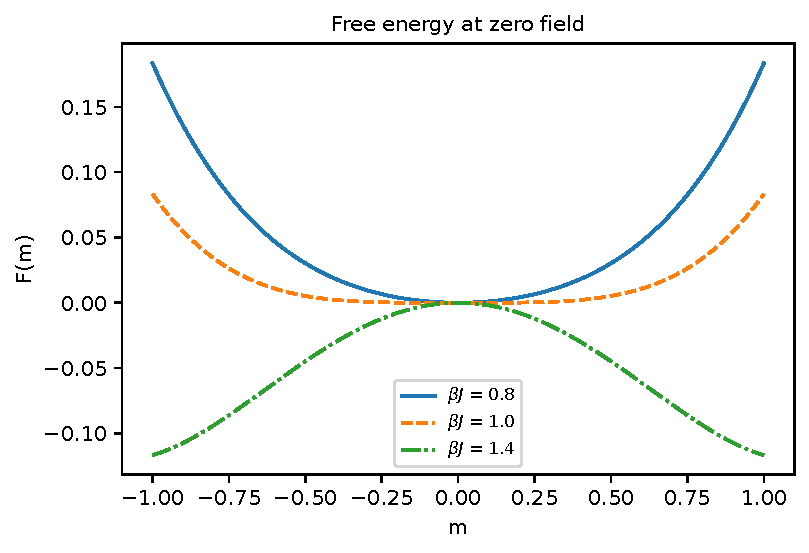
\includegraphics[width=0.7\textwidth]{F1_free_energy.pdf}
\caption{Free energy, Eq.~\eqref{eq:landau}, at zero field for $\beta J = 0.8$, $1.0$ and
$1.4$ with the coefficients of Eq.~\eqref{eq:coefficients}. The double well appears only above
$\beta J = 1$.}
\label{fig:free-energy}
\end{figure}

The quartic is used here for the qualitative structure and the exponents. The spinodal field
of Section~\ref{sec:spinodal} is computed from the full Eq.~\eqref{eq:selfcons}, not from the
truncated quartic, which reproduces it only as $\beta J \to 1^+$.

The linear response to the reduced field is
\begin{equation}
\chi \equiv \frac{\partial m}{\partial h}
     = \frac{\operatorname{sech}^2(\beta J m^\ast + h)}
            {1 - \beta J \operatorname{sech}^2(\beta J m^\ast + h)},
\label{eq:chi}
\end{equation}
so that the response to the unreduced field is $\partial m/\partial H = \beta\chi$. It
diverges where the denominator vanishes; we report $\chi$ only on stable roots, where the
denominator is positive.

\section{Results}
\label{sec:results}

\subsection{Numerical validation against the exact exponents}
\label{sec:numerics}

Every later figure is drawn with the same solver, so the solver is checked first against
results that are known exactly. Mean-field theory gives \cite{goldenfeld1992}
\begin{equation}
\beta = \tfrac{1}{2}, \qquad \gamma = 1, \qquad \delta = 3,
\end{equation}
for $m^\ast \sim (\beta J - 1)^{\beta}$ at zero field, $\chi \sim |1 - \beta J|^{-\gamma}$,
and $m \sim h^{1/\delta}$ on the critical isotherm $\beta J = 1$. (The exponent $\beta$ is not
to be confused with the inverse temperature; context distinguishes them.) All three follow
directly from Eq.~\eqref{eq:stationarity}: $m^{\ast 2} = 3(\beta J - 1)$ at zero field,
$\chi = 1/(1 - \beta J)$ at $m^\ast = 0$, and $m^3 = 3h$ at $\beta J = 1$.

One methodological point matters. Solving Eq.~\eqref{eq:selfcons} by direct iteration of
$m_{k+1} = \tanh(\beta J m_k + h)$ is the natural implementation and is adequate away from
criticality, but its convergence degrades at $\beta J = 1$, where the map's derivative
reaches unity. The exponents are defined in that limit, so fitting them to iterated values
measures truncation error rather than physics: with $10^3$ iterations and tolerance
$10^{-10}$, doing so returns $\delta \approx 1.35$ against an exact $3$. We therefore fit the
exponents to roots obtained by bracketing, and check the iterative solver against the
bracketed one away from criticality ($|\beta J - 1| \ge 0.02$), where the largest absolute
discrepancy over the sampled grid is $\pbSolverAgreement$.

Fitting $\beta$ and $\gamma$ at $\pbFitPoints$ points in a window of width $\pbFitWindow$ in
$|\beta J - 1|$, and $\delta$ at $\pbFitPoints$ log-spaced fields $10^{-6} \le h \le
10^{-3}$, recovers
\begin{equation}
\beta = \pbBetaFitted, \qquad \gamma = \pbGammaFitted, \qquad \delta = \pbDeltaFitted,
\end{equation}
with absolute errors $\pbBetaError$, $<10^{-14}$ and $\pbDeltaError$ respectively. The $\gamma$
fit is exact by construction, since $m^\ast = 0$ below the transition at zero field and
$\chi = 1/(1-\beta J)$ identically; it checks the susceptibility expression and the fitting
procedure rather than the root finder. The residual error in $\beta$ is a correction to
scaling: keeping the next term of the expansion, $m^5/5$, gives
$m^{\ast 2} = 3t\,(1 - \tfrac{9}{5}t + O(t^2))$ with $t = \beta J - 1$, which lowers the
effective log-log slope across a finite window. Figures~\ref{fig:order}, \ref{fig:chi} and
\ref{fig:isotherm} show the three fits.

\begin{figure}[htbp]
\centering
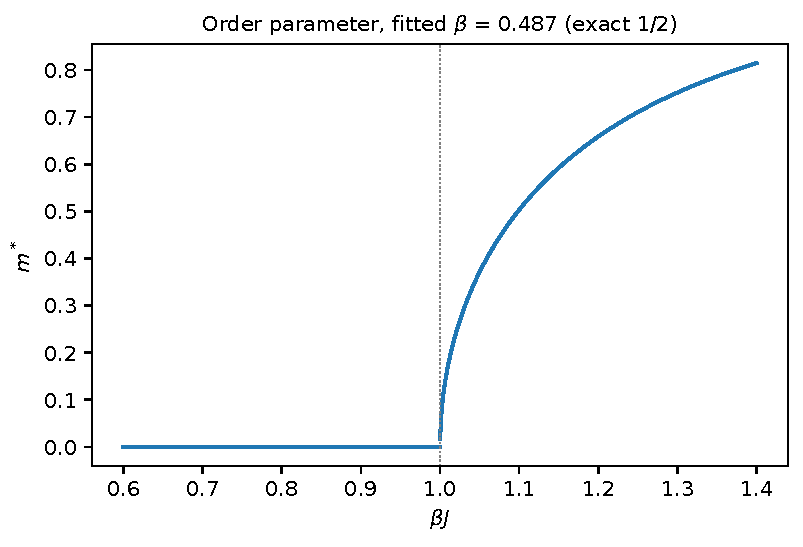
\includegraphics[width=0.7\textwidth]{F2_order_parameter.pdf}
\caption{Order parameter across the transition. The fitted exponent is $\pbBetaFitted$
against an exact $1/2$.}
\label{fig:order}
\end{figure}

\begin{figure}[htbp]
\centering
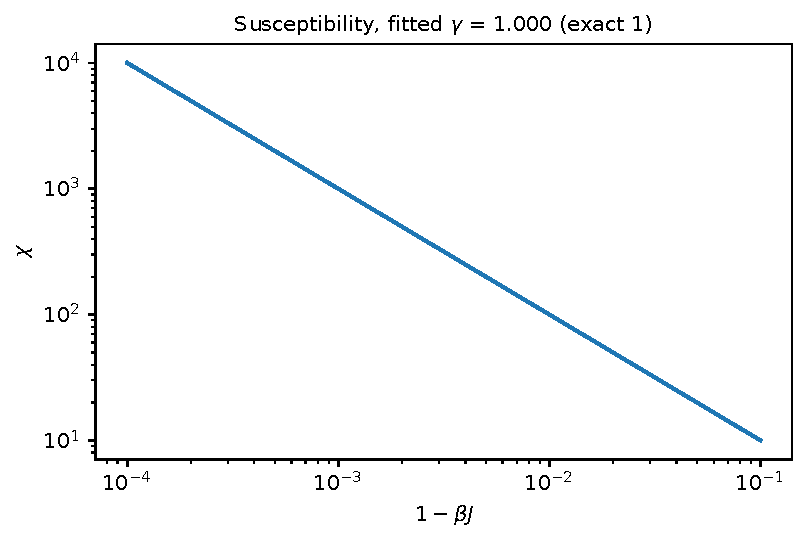
\includegraphics[width=0.7\textwidth]{F3_susceptibility.pdf}
\caption{Susceptibility, Eq.~\eqref{eq:chi}, approaching criticality from below at zero
field; fitted exponent $\pbGammaFitted$ against an exact $1$.}
\label{fig:chi}
\end{figure}

\begin{figure}[htbp]
\centering
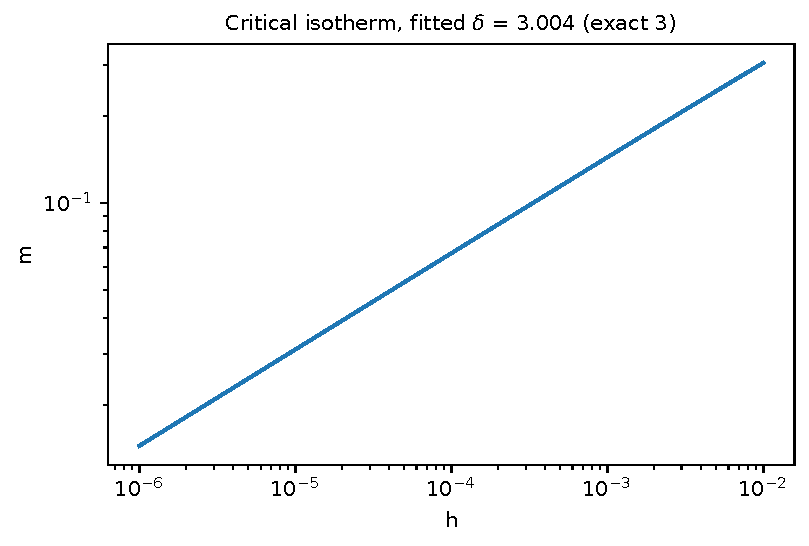
\includegraphics[width=0.7\textwidth]{F4_critical_isotherm.pdf}
\caption{Critical isotherm at $\beta J = \pbCriticalBetaJ$, fitted exponent
$\pbDeltaFitted$ against an exact $3$.}
\label{fig:isotherm}
\end{figure}

\subsection{The spinodal field}
\label{sec:spinodal}

Above $\beta J = 1$ the free energy has two minima at zero field. A field deepens one and
shallows the other; at a finite field the shallower minimum disappears. That value is the
spinodal field $h_c(\beta J)$: the field a population in the metastable state must experience
before, within mean-field theory, it is obliged to move.

It follows in closed form from Eq.~\eqref{eq:selfcons}. Write the roots as solutions of
$h = g(m) \equiv \operatorname{artanh}(m) - \beta J m$. A pair of roots merges and disappears
where $g'(m) = 1/(1-m^2) - \beta J = 0$, that is at
\begin{equation}
m_s^2 = 1 - \frac{1}{\beta J},
\label{eq:ms}
\end{equation}
and the corresponding field is
\begin{equation}
h_c(\beta J) = \big|\operatorname{artanh}(m_s) - \beta J m_s\big|
             = \beta J m_s - \operatorname{artanh}(m_s).
\label{eq:hc}
\end{equation}
At $\beta J = 2$, $m_s = 1/\sqrt{2}$ and $h_c = \sqrt{2} - \operatorname{artanh}(1/\sqrt{2})
= \pbHcAtMax$. As $\beta J \to 1^+$, Eq.~\eqref{eq:hc} gives
$h_c \simeq \tfrac{2}{3}(\beta J - 1)^{3/2}$, the value the quartic of
Eq.~\eqref{eq:landau} predicts; away from the transition the quartic overestimates it
($2/3$ against $\pbHcAtMax$ at $\beta J = 2$). The figures are drawn from a bisection on the
number of stable roots of Eq.~\eqref{eq:selfcons}, which agrees with Eq.~\eqref{eq:hc} to
better than $10^{-6}$ over the plotted range. Figure~\ref{fig:phase} shows the boundary;
$h_c$ vanishes as $\beta J \to 1^+$ and increases monotonically with $\beta J$.

\begin{figure}[htbp]
\centering
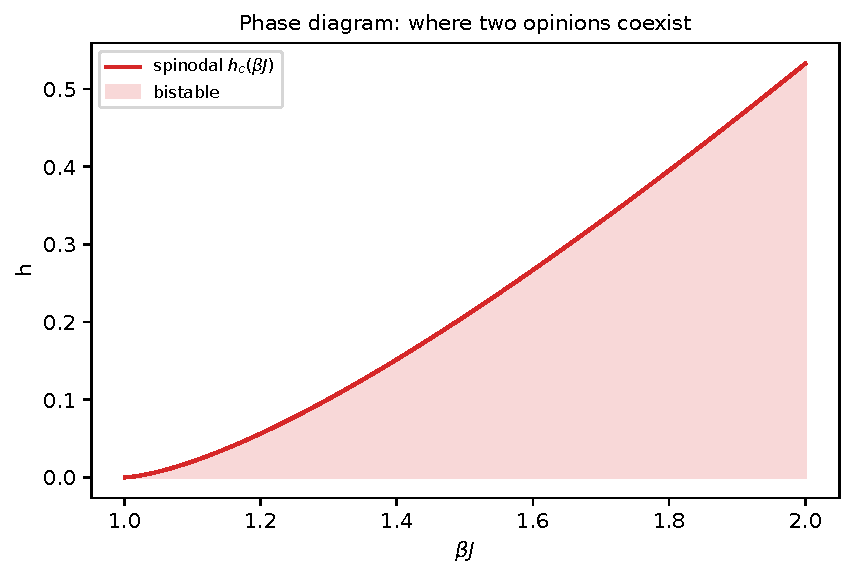
\includegraphics[width=0.7\textwidth]{F5_phase_diagram.pdf}
\caption{Phase diagram in $(\beta J, h)$ for $h \ge 0$; the diagram is symmetric under
$h \to -h$. The shaded region is where two stable opinion states coexist; its upper boundary
is the spinodal $h_c(\beta J)$ of Eq.~\eqref{eq:hc}.}
\label{fig:phase}
\end{figure}

\subsection{The bound}
\label{sec:bound}

Now let the field be generated by a content observable. Any such proposal has the form
\begin{equation}
h = \alpha X,
\end{equation}
where $X$ is measurable on a piece of content and $\alpha$ is an unknown coupling carrying
the units. Real observables are bounded: across the content a population plausibly
encounters, $X$ lies in some interval $[X_{\min}, X_{\max}]$ of width
$\Delta X = X_{\max} - X_{\min}$, which is an empirical property of the observable and of the
corpus, not of the model.

Two further assumptions fix the reference point. First, the field is measured from the
content-free reference $h = 0$, at which the population sits in one of the two symmetric
states $\pm m^\ast$. Second, $X$ is signed about a neutral value $X = 0$ that lies inside the
attainable range, $X_{\min} \le 0 \le X_{\max}$, as for an observable defined as a difference
between two opposing components. Then every attainable field satisfies
$|h| \le |\alpha| \max(|X_{\min}|, |X_{\max}|) \le |\alpha|\,\Delta X$. Moving a population
from either state into the other through a spinodal crossing requires a field of magnitude at
least $h_c(\beta J)$ opposing that state, so a necessary condition is
\begin{equation}
|\alpha|\, \Delta X \;\ge\; h_c(\beta J)
\qquad \Longleftrightarrow \qquad
|\alpha| \;\ge\; \frac{h_c(\beta J)}{\Delta X}.
\label{eq:bound}
\end{equation}
Replacing $\Delta X$ by $\max(|X_{\min}|, |X_{\max}|)$ gives a tighter condition; the form in
Eq.~\eqref{eq:bound} is the weaker one and so remains necessary under the stated assumptions.
Figure~\ref{fig:alpha} plots the right-hand side against $\beta J$ for several values of
$\Delta X$. At $\beta J = \pbBetaJMax$ the required coupling is $\pbAlphaRequiredOneTenth$ for
an observable of spread $0.1$, $\pbAlphaRequiredHalf$ for spread $0.5$,
$\pbAlphaRequiredUnity$ for unit spread and $\pbAlphaRequiredDouble$ for spread $2$.

\begin{figure}[htbp]
\centering
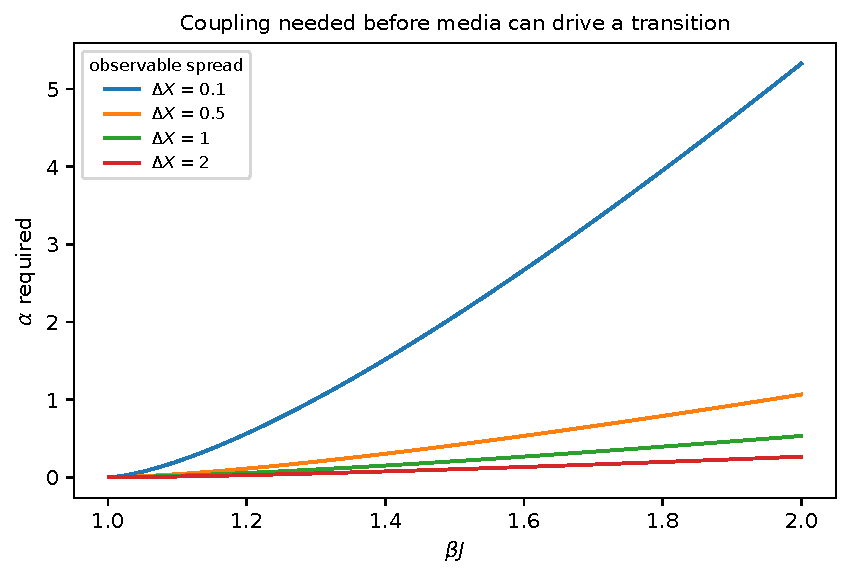
\includegraphics[width=0.7\textwidth]{F6_alpha_required.pdf}
\caption{Coupling $h_c(\beta J)/\Delta X$ required before a content observable of spread
$\Delta X$ can drive the population across the spinodal, Eq.~\eqref{eq:bound}.}
\label{fig:alpha}
\end{figure}

Three properties of Eq.~\eqref{eq:bound} are worth drawing out.

First, it is a necessary condition, not a sufficient one. Clearing the bound does not
establish that content moves populations; it only fails to rule it out. Falling below it
excludes the mechanism within the model's assumptions, for a population that must cross the
spinodal.

Second, it does not require the coupling to be estimated. $\Delta X$ is obtained by measuring
the observable across a corpus, which does not need the outcome variable and is ordinarily far
cheaper than estimating a coupling to collective behaviour, and $h_c$ comes from the model.

Third, it turns a null result into a quantitative constraint. A study that estimates $\alpha$
and obtains an interval containing zero has, on its own, only the statement that no coupling
was detected. Combined with Eq.~\eqref{eq:bound}, the same interval states that the coupling
would have to exceed $h_c(\beta J)/\Delta X$ for the mechanism to operate, and whether the
measurement excludes that range at the stated confidence. This is available to any study that
reports a spread alongside its estimate.

As an illustration, a companion study by the author (manuscript in preparation) measures a
signed neural-response observable on a 400-article corpus and finds a range that contains
zero, with spread $\Delta X = 0.1241$. Equation~\eqref{eq:bound} then requires
$|\alpha| \ge \pbHcAtMax/0.1241 \approx 4.29$ at $\beta J = 2$. This is a statement about
what the coupling would have to be, not a measurement of it.

\section{Discussion}
\label{sec:discussion}

\subsection{A screening criterion}
\label{sec:screening}

The bound supports a procedure that can be run before outcome data are collected.

\begin{enumerate}
\item State the observable $X$ and the map $h = \alpha X$ explicitly, including units, and
the neutral value $X = 0$.
\item Measure or bound $\Delta X$ on a sample of the content of interest, and check that the
range contains the neutral value. This does not require the outcome variable.
\item Choose the range of $\beta J$ the population plausibly occupies and evaluate
$h_c(\beta J)$ from Eq.~\eqref{eq:hc}.
\item Evaluate $\alpha_{\min} = h_c(\beta J)/\Delta X$ and ask whether a coupling of that
size is defensible on independent grounds.
\item If it is not, the mechanism is excluded within the model and the expensive measurement
is unnecessary. If it is, proceed, and report $\Delta X$ alongside the estimate of $\alpha$
so that the bound can be applied to the result.
\end{enumerate}

The weakest link is step 4, since $\alpha$ has no independent scale in most applications. The
criterion is still informative in relative terms: candidate observables can be ranked by
$\alpha_{\min}$, provided they are first expressed on a common scale (for example, each
standardised by its own standard deviation across the corpus), since rescaling an observable
by a constant rescales $\alpha_{\min}$ by its inverse. An observable whose spread demands an
implausibly large coupling is a poor choice of field regardless of how well it correlates with
anything.

\subsection{Scope and limitations}
\label{sec:limitations}

The result inherits every assumption of the all-to-all mean-field model: a single homogeneous
population, a static field, binary opinions, and the thermodynamic limit. On sparse or
finite-dimensional networks, with heterogeneous susceptibility, or with temporal dynamics,
the switching field differs from Eq.~\eqref{eq:hc}, so Eq.~\eqref{eq:bound} is a bound within
this model rather than a universal one. The linear map $h = \alpha X$ is the simplest possible
coupling and is an assumption in its own right; a saturating map would change the relation
between $\Delta X$ and the maximum attainable field. The reference-point assumptions matter
too: if the content-free field is not zero but already favours the target state by $h_0 > 0$,
the requirement relaxes to $|\alpha|\Delta X \ge h_c - h_0$, and if the attainable range of
$X$ does not contain its neutral value the maximum field is no longer bounded by
$|\alpha|\Delta X$. Finally, the spinodal is the relevant threshold for a population trapped
in a metastable state. In the all-to-all model at $N \to \infty$ the metastable state does not
decay below $h_c$, but a finite population, or one on a network, can escape by activated
nucleation at smaller fields given enough time; Eq.~\eqref{eq:bound} then demands more of
$\alpha$ than a nucleation argument would, and can overstate the coupling required. The bound
does not measure $\alpha$ and does not predict that media content moves opinion.

\section{Conclusion}
\label{sec:conclusion}

In all-to-all mean-field Ising opinion dynamics with a content-driven field $h = \alpha X$,
a population starting from the symmetric zero-field state cannot be carried across the
spinodal by content unless $|\alpha| \ge h_c(\beta J)/\Delta X$, with $h_c$ given in closed
form by Eq.~\eqref{eq:hc}. The condition is necessary, not sufficient; it needs only the
measured spread of the observable and the model's spinodal, so it can screen a proposed
mechanism before outcome data exist, and it turns a null estimate of the coupling into a
statement about the range that estimate excludes. Extending the bound to networked,
heterogeneous and finite populations, where nucleation replaces the sharp spinodal, is the
natural next step.

\section*{Data availability}

No empirical data were used; the paper is analytic and numerical. All figures and every
number quoted are produced by
\nolinkurl{services/inference/scripts/phase_boundary.py}, which also enforces the exponent check (it exits non-zero if any fitted exponent departs from
its exact value by more than a stated tolerance), and are written into the manuscript by
\nolinkurl{services/inference/scripts/paper1_numbers.py} rather than transcribed. The code and
the generated records are public at \url{https://github.com/brn-mwai/monarch}.

\section*{CRediT authorship contribution statement}

\textbf{Brian Mwai:} Conceptualization, Methodology, Software, Validation, Formal analysis,
Investigation, Visualization, Writing -- original draft, Writing -- review \& editing.
% If co-authorship is agreed, add:
% \textbf{Songa Mutambi:} Supervision, Writing -- review \& editing.

\section*{Declaration of competing interest}

The author declares no known competing financial interests or personal relationships that
could have appeared to influence the work reported in this paper.

\section*{Funding}

This research did not receive any specific grant from funding agencies in the public,
commercial, or not-for-profit sectors.

\section*{Declaration of generative AI and AI-assisted technologies in the writing process}

During the preparation of this work the author used Claude (Anthropic), an AI assistant, for
editing the manuscript and for support in writing and checking analysis code. After using
this tool, the author reviewed and edited the content as needed and takes full responsibility
for the content of the publication.

\section*{Acknowledgements}

The author thanks Dr.\ Songa Mutambi, Department of Natural Sciences, The Catholic University
of Eastern Africa, for supervising the project of which this work forms part, and for
suggesting the signed-difference form of the observable used in the companion study.

\begin{thebibliography}{11}

\bibitem{castellano2009}
C.~Castellano, S.~Fortunato, V.~Loreto,
Statistical physics of social dynamics,
Rev. Mod. Phys. 81 (2009) 591--646. \href{https://doi.org/10.1103/RevModPhys.81.591}{https://doi.org/10.1103/RevModPhys.81.591}.

\bibitem{galam2008}
S.~Galam,
Sociophysics: a review of Galam models,
Int. J. Mod. Phys. C 19 (2008) 409--440. \href{https://doi.org/10.1142/S0129183108012297}{https://doi.org/10.1142/S0129183108012297}.

\bibitem{sznajd2000}
K.~Sznajd-Weron, J.~Sznajd,
Opinion evolution in closed community,
Int. J. Mod. Phys. C 11 (2000) 1157--1165. \href{https://doi.org/10.1142/S0129183100000936}{https://doi.org/10.1142/S0129183100000936}.

\bibitem{stauffer2008}
D.~Stauffer,
Social applications of two-dimensional Ising models,
Am. J. Phys. 76 (2008) 470--473. \href{https://doi.org/10.1119/1.2779882}{https://doi.org/10.1119/1.2779882}.

\bibitem{crokidakis2012}
N.~Crokidakis,
Effects of mass media on opinion spreading in the Sznajd sociophysics model,
Physica A 391 (2012) 1729--1734. \href{https://doi.org/10.1016/j.physa.2011.11.038}{https://doi.org/10.1016/j.physa.2011.11.038}.

\bibitem{azhari2023}
Azhari, R.~Muslim,
The external field effect on the opinion formation based on the majority rule and the
$q$-voter models on the complete graph,
Int. J. Mod. Phys. C 34 (2023) 2350088. \href{https://doi.org/10.1142/S0129183123500882}{https://doi.org/10.1142/S0129183123500882}.

\bibitem{freitas2020}
F.~Freitas, A.~R. Vieira, C.~Anteneodo,
Imperfect bifurcations in opinion dynamics under external fields,
J. Stat. Mech. Theory Exp. 2020 (2020) 024002. \href{https://doi.org/10.1088/1742-5468/ab6848}{https://doi.org/10.1088/1742-5468/ab6848}.

\bibitem{sirbu2016}
A.~S\^{i}rbu, V.~Loreto, V.~D.~P. Servedio, F.~Tria,
Opinion dynamics: models, extensions and external effects,
in: V.~Loreto, et al. (Eds.), Participatory Sensing, Opinions and Collective Awareness,
Understanding Complex Systems, Springer, Cham, 2017, pp. 363--401.
\href{https://doi.org/10.1007/978-3-319-25658-0_17}{https://doi.org/10.1007/978-3-319-25658-0\_17}.

\bibitem{mullick2025}
P.~Mullick, P.~Sen,
Sociophysics models inspired by the Ising model,
Eur. Phys. J. B 98 (2025) 206. \href{https://doi.org/10.1140/epjb/s10051-025-01053-7}{https://doi.org/10.1140/epjb/s10051-025-01053-7}.

\bibitem{korbel2026}
J.~Korbel, R.~Dahdoul, S.~Thurner,
Empirical validation of the polarization transition in a double-random field model of
elections,
Phys. Rev. Lett. 136 (2026) 127402. \href{https://doi.org/10.1103/9gjj-1df6}{https://doi.org/10.1103/9gjj-1df6}.

\bibitem{goldenfeld1992}
N.~Goldenfeld,
Lectures on Phase Transitions and the Renormalization Group,
Addison-Wesley, Reading, MA, 1992.

\end{thebibliography}

\end{document}
